%%%%%%%%%%%%%%%%%%%%%%%%%%%%%%%%%%%%%%%%%
% Reporte de prácticas
% Ingeniería Informática
% LaTeX Template
% Version 0.1 (27/09/20)
% Original author: Abraham Marianjel Sepúlveda
%%%%%%%%%%%%%%%%%%%%%%%%%%%%%%%%%%%%%%%%%%
\documentclass[12pt,letterpaper]{article} 
\usepackage[utf8]{inputenc} 
\usepackage[spanish, es-tabla, es-nodecimaldot]{babel} % Formato a español
\usepackage[T1]{fontenc}    % Permite utilizar otras tipografías
\usepackage[vmargin=2.5cm,hmargin=2.5cm]{geometry}
\usepackage{multicol}   % Unir columnas en tablas y formato a dos columnas
\usepackage{multirow}   % Unir filas en tablas
\usepackage{graphicx}   % Necesario para insertar gráficas
\usepackage{float}      % Corregir ubicación de imágenes y tablas
%\usepackage{subfigure} % Insertar subfiguras
\usepackage{url}       % Hiervínculo a direcciones URL
\usepackage{cite}
\usepackage{lscape} % Para poner una unica hoja en horizontal
\usepackage{listings}
\usepackage{flushend}
\usepackage[none]{hyphenat} % Permite utilizar el comando \sloppy
\usepackage[small]{caption}	% Reduce el tamaño de letra utilizado en los pies de figura.
\usepackage{hyperref}   % Agrega enlaces internos de las secciones, figuras y tablas.
\usepackage{color}      % Definición de colores
    \hypersetup{colorlinks=true, linkcolor=[rgb]{0,0,1}, citecolor=[rgb]{0,0,1}}
\usepackage{xcolor}		% Permite definir un color para utilizarlo dentro del documento.
    \definecolor{gris}{RGB}{70,70,70}	% Definiendo el color gris
    \definecolor{negro}{RGB}{40,40,40}		% Definiendo el color negro

%%%%%%%% Modificación de los espacios de los títulos de secciones %%%%%%%%%%
%======================================================================================
\usepackage{titlesec}		% Permite reconfigurar  los títulos de las secciones y subsecciones
%\renewcommand\thesection{\Roman{section}}	% Numeración romana en las secciones
\renewcommand\thesubsection{\Roman{subsection}}		% Numeración romana en las subsecciones
\titlespacing*{\section}{0pt}{2.5mm}{0mm}	% Espaciado del título {espacio izquierdo}{arriba del título}{abajo del título}
\titleformat{\section}[block]{\large\scshape\centering}{\thesection.}{1em}{}	% Espaciado del título de las secciones
\titleformat{\subsection}[block]{\large}{\thesubsection.}{1em}{}				% Espaciado del título de las subsecciones
%%%%%%%%%%%%%%%%%%%%%%%%%%%%%%%%%%%%%%%%%%%%%%%%%%%%%%%%%%%%%%%%%%%%%%%%%%%%%%

%Se define un comando \colorhrule para hacer líneas horizontales de color con 3 argumentos: color, largo, ancho.
\newcommand{\colorhrule}[3]{\begingroup\color{#1}\rule{#2}{#3}\endgroup}

\setlength{\intextsep}{1mm} % Distancia superior e inferior en objetos flotantes
\setlength{\columnsep}{5mm} % Separación entre columnas del documento
%**************************************Encabezado****************************************
%=========================================================================================
\begin{document}
\sloppy     % Evita que las palabras se corten al saltar de línea.
\begin{center}
	\begin{tabular}{cc}
	\multirow{2}{3.5cm} {
\includegraphics[scale=0.3]{../../../Logos FACE/logosimbologia.png}   }	& \huge{\textsc{\textbf{Universidad del Bio Bio}}}\\ %\vspace{5mm}
 & \scriptsize{\textsc{Facultad de Ciencias Empresiariales}}\\[4mm]% Sele puede cambiar al LARGE
 & \Large{\textsf{\textbf{Guía BPMN}}}\\
 & \small Profesor: {\textsf{Luis Rojas}}\\
 & \small Ayudante: {\textsf{Abraham Marianjel}}\\

 & \small{\textsc{Ingeniería Civil en Informática $|$ Modelamiento}}\\
 & \today\\
	\end{tabular}
\end{center}
\begin{center}
\colorhrule{negro}{16.5cm}{1.2pt}
\end{center}

\begin{abstract}
\noindent \par BPMN es una notación gráfica para el modelado de procesos. Como componente central de BPM, permite a las organizaciones, independientemente del tamaño de la empresa o la industria, visualizar y optimizar sus procesos de negocio. Mediante el uso de este lenguaje de modelado, los pasos de trabajo se representan de forma consistente y, por lo tanto, fácilmente comprensible para todos los participantes en el proceso. Por lo tanto, la comunicación de los procesos se simplifica en toda la organización. El BPMN fue desarrollado en 2001. En el curso de numerosas revisiones, el Grupo de Gestión de Objetos® (OMG) publicó BPMN 2.0 en 2010. El metamodelo también contiene una semántica de ejecución que puede ser usada para la automatización técnica usando un motor de procesos. 
\end{abstract}
\begin{center}
\vspace{-5mm}
\colorhrule{gris}{16.5cm}{0.7pt}
\end{center}
%*******************************Texto del Informe*********************************************
%==============================================================================================

\par \textsc{Descripción:} \textit{El modelado de los procesos en BPMN permite la representación eficiente de los procesos de negocio. Si quiere crear un diagrama en BPMN, primero tiene que crear una piscina, que puede dividir en varios carriles. También es posible modelar múltiples piscinas, dependiendo del tipo de diagrama seleccionado. El modelado de procesos siempre comienza con al menos un evento de inicio y termina con uno o más eventos finales. El proceso creado en el ínterin consiste en eventos, actividades, compuertas y, si es necesario, artefactos adicionales. Las reglas de modelado específicas aseguran el uso correcto de los elementos y la documentación uniforme de los procesos.}\vspace{2cm}

\section*{\LARGE\textbf{ Actividades}}
\textit{En las actividades a desarrollar esta la replicación y la interpretación del proceso de negocios, modelandolo con herramientas digitales o en su cuaderno.}\\

\subsection{\textbf{Replicación Tienda en Linea}}
Se necesita que los alumnos copien el siguiente diagrama para poder entender la dirección de las ordenes del proceso de negocios y que hacer con los eventos, tareas y mensajes.\\


\begin{landscape}

	\begin{figure}[H]
		\centering
		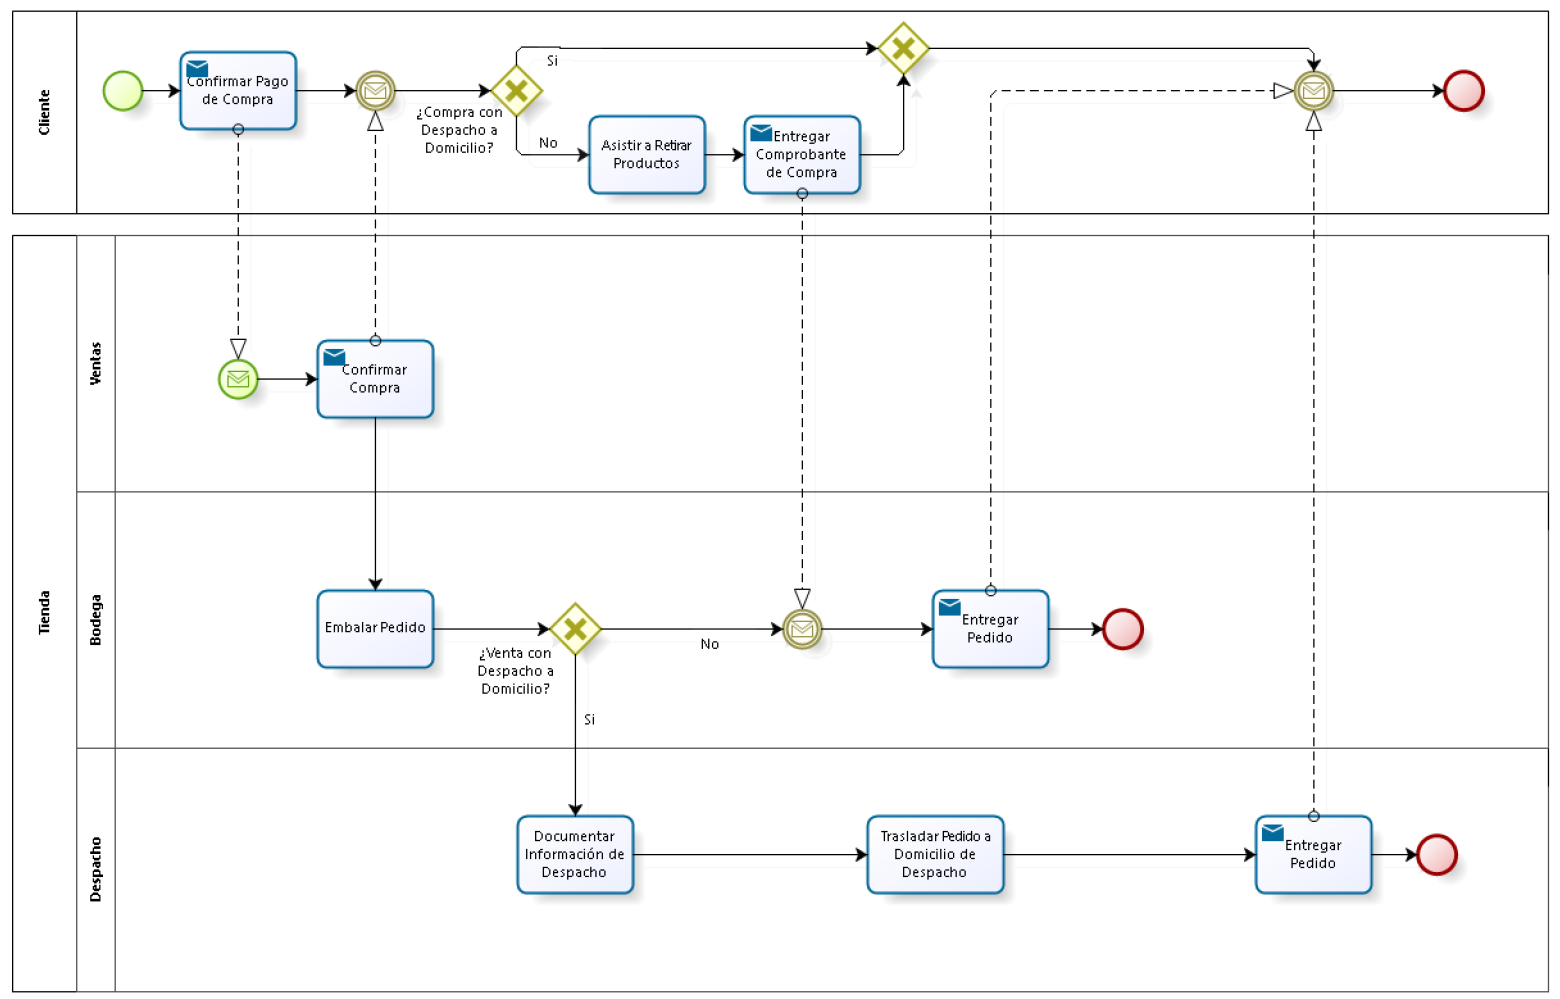
\includegraphics[scale=0.55]{img/tienda en linea.PNG}    
		\caption{Tienda en linea con BPMN }
	\label{fig:rc}
	\end{figure}

\end{landscape}
	
\subsection{\textbf{Proceso de Evaluación}}
El profesor encargado de las clases prácticas se encuentra muy preocupado por mantener un claro proceso para la preparación, realización y evaluación de cada clase. Con el objetivo de que este proceso sea conocido por sus estudiantes, al profesor se le ha ocurrido la idea de encargarles a éstos que modelen el proceso utilizando Bizagi.
\par La primera actividad que debe realizar el profesor siempre es preparar las tareas que deberán realizar los estudiantes. Luego, en caso de que las tareas sean evaluadas, el profesor se encarga de generar la pauta de evaluación correspondiente. Finalmente, el profesor crea una presentación con los enunciados de las tareas y la pauta de evaluación.
\par Una vez preparada, el profesor puede realizar la clase, la cual normalmente consiste en tres actividades secuenciales: presentar la herramienta con la que se trabajar á , realizar un ejercicio de ejemplificación, y entregar las tareas a realizar por los estudiantes. Paralelamente a las actividades anteriores, el profesor siempre se mantiene dispuesto a contestar las dudas de los estudiantes.
\par Luego de finalizar la clase, el proceso acaba si ésta no poseía tareas evaluadas. En caso contrario, el profesor debe revisar las entregas de los estudiantes y luego notificarles sus calificaciones.\\

\subsection{\textbf{Contratación de Personal}}	
El proceso de contratación de personal para dictar asignaturas en la carrera de Ingeniería Civil en Informática es una labor que se realiza al inicio de todos los semestres Esto procesa las solicitudes de contratación que emite el programa de ICI en base a las asignaturas que corresponde dictar En el proceso de organización, la Dirección de ICI ha decidido documentar de manera formal el proceso, y así obtener un modelo de negocios descrito en BPMN que permita facilitar la comprensión del proceso en cuestión.
\par En el proceso de contratación intervienen diferentes áreas el Departamento de Pregrado, Dirección de ICI, el Departamento de Personal y Contralor í a Todo comienza con la solicitud que se envía desde la Dirección de ICI al Departamento de Pregrado para solicitar la contratación de un profesional Este departamento revisa la solicitud y, de ser necesarias algunas modificaciones, las solicita para que la Dirección de ICI las corrija y reenvíe la solicitud Si no hay modificaciones, se autoriza y notifica a la Dirección de ICI Luego, desde la Dirección de ICI se debe firmar la solicitud y enviarla al Departamento de Personal para que ellos la analicen En el Departamento de Personal se revisa el documento, siendo posible que realicen observaciones para modificarlo Si hay observaciones, el documento debe ser modificado y comenzar todo el proceso nuevamente, en otro caso, el Departamento de Personal notifica la solicitud de firma al profesional y a la Dirección de ICI Posteriormente, cuando el profesional ha firmado el convenio de servicios, el documento debe ser enviado a Contralor í a para que sea decretado, con lo que se finaliza el proceso.\\




	\subsection{\textbf{Sistema de organización en Campeonatos Federados de Voleibol}}	
	Convertir utilizando 2 pool en vez de 2 line.
	
	\begin{figure}[H]
		\centering
		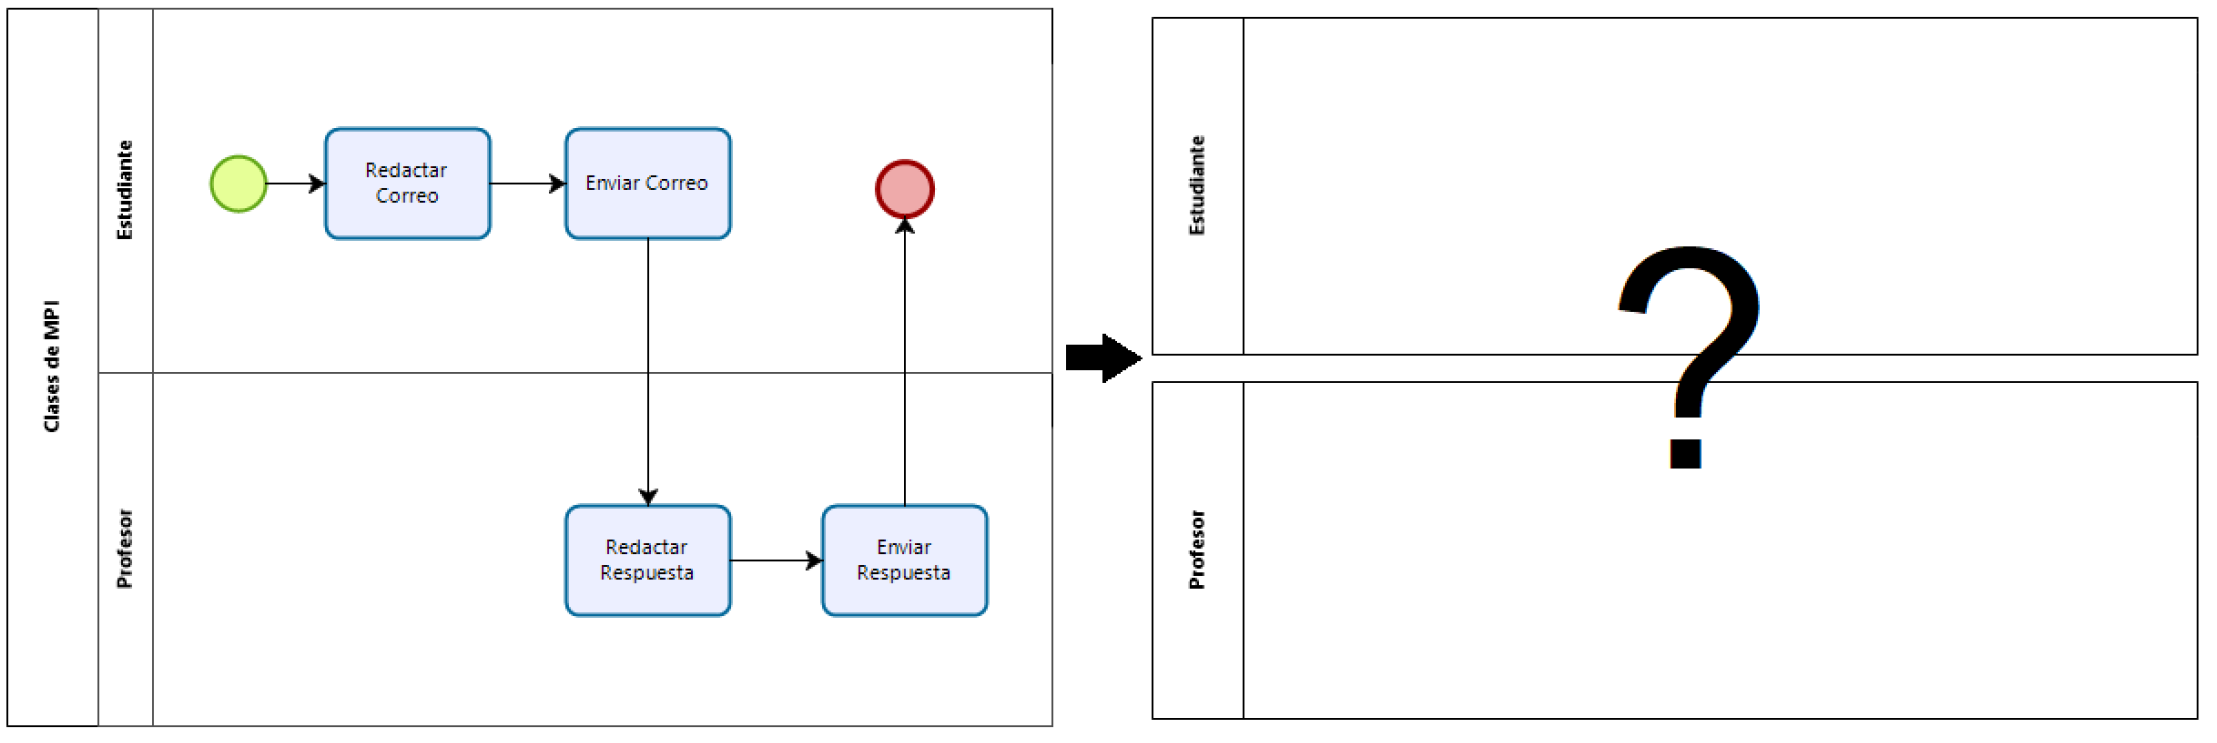
\includegraphics[scale=0.25]{img/2pool.PNG}     
		\caption{2 Pool }
	\label{fig:rc}
	\end{figure}

	\subsection{\textbf{Sistema de organización en Campeonatos Federados de Voleibol}}
	Análizar y redactar el proceso de negocios que se muestra en la imágen de Sistema de Organización de Voleibol
	
	\begin{figure}[H]
		\centering
		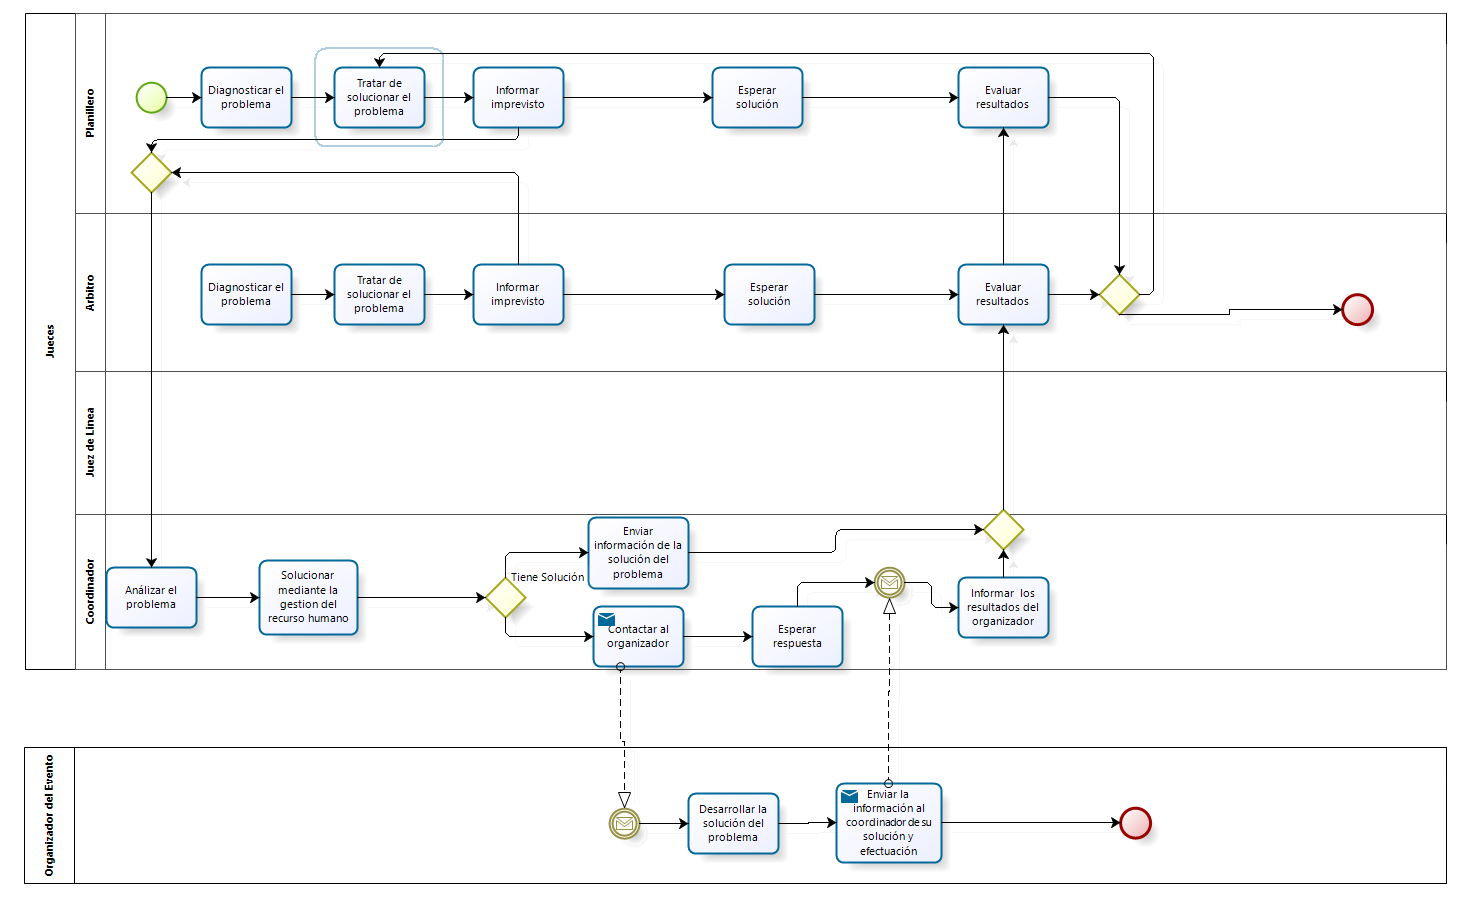
\includegraphics[scale=0.43]{img/campeonato.PNG}      
		\caption{Sistema de Organización de competencia }
	\label{fig:rc}
	\end{figure}

\end{document}
